%Marco Teórico

\section{Estimulación eléctrica funcional}
La estimulación eléctrica funcional es la aplicación de corriente eléctrica a tejido excitable para suplementar o reemplazar funciones que se han perdido en individuos con daños neurológicos. El propósito de la intervención FES es habilitar funciones que se han perdido en individuos con daño al sistema nervioso mediante la sustitución o asistencia a las habilidades voluntarias de dichos individuos. En las aplicaciones FES la estimulación es requerida para lograr una función deseada, por lo tanto, los sistemas FES usualmente se diseñan para ser controlados a partir de señales relacionadas a la actividad o intención del propio usuario. Los dispositivos FES que son usados para sustituir una función neurológica que se ha perdido son comúnmente llamadas neuroprótesis \cite{Peckham2005}.

\section{Neuroprótesis}
Una neuroprótesis es un dispositivo que proporciona ráfagas cortas de impulsos eléctricos al sistema nervioso central o periférico a través de electrodos superficiales, para lograr producir funciones sensoriales o motoras. Estos dispositivos buscan sustituir o asistir una función dañada debido a una lesión o enfermedad en el sistema nervioso \cite{Popovic2008}\cite{Popovic2015}.

En general, existen dos tipos de neuroprótesis: a) las neuroprótesis autónomas, las cuales son sistemas autocontenidos que imitan las funciones de una contraparte biológica, y b) las neuroprótesis por comando, las cuales son sistemas que reemplazan o asisten una función sensitiva o motora que se ha perdido o disminuido. Estas últimas están compuestos por un sistema de control que interpreta la intención del usuario, utilizan sensores para detectar el estado del sistema, genera la activación del sistema motor o sensorial del usuario, y proporciona una retroalimentación al usuario \cite{Popovic2015}.

Las neuroprótesis motoras, las cuales son un ejemplo de neuroprótesis por comando, son sistemas que asisten a personas que han sufrido algún tipo de lesión en la médula espinal o cerebro. Estas neuroprótesis pueden actuar directamente en el sistema nervioso central, en el sistema nervioso periférico o bien, en una combinación de ambos \cite{Popovic2015}.

\section{Señales de comando y retroalimentación}
Como se muestra en la Figura \ref{Figura: CompNeuroP}, una neuroprótesis por comando requiere de dos señales esenciales para lograr su correcto funcionamiento, una de estas es una señal de comando y otra es una señal de retroalimentación \cite{Popovic2015}.

\begin{figure}[htbp]
\centering
	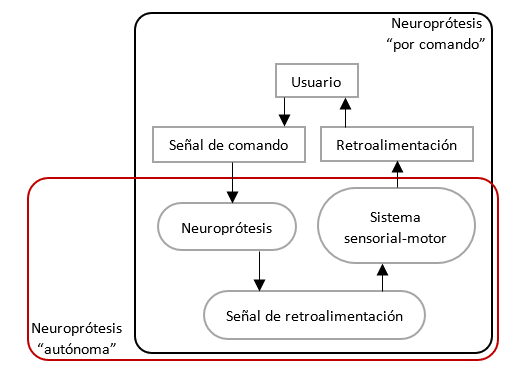
\includegraphics[scale=0.8]{CompNeuroP_ESP.png}
	\caption{Esquema de los componentes generales de una neuroprótesis autónoma y por comando. Adaptado de \cite{Popovic2015}.}
	\label{Figura: CompNeuroP}
\end{figure}

\subsection{Señal de comando}
Son señales utilizadas como indicadores de eventos de determinada tarea. En el caso de las neuroprótesis son las señales que controlan las acciones de esta, especialmente las acciones relacionadas a la estimulación eléctrica (inicio, fin, incremento de intensidad, disminución de intensidad, etc.).

\subsection{Señal de retroalimentación}
Es un tipo de señal que brinda al sistema información relacionada a la respuesta a un determinado comando. Estas señales, en el caso de las neuroprótesis, suelen estar relacionadas con el monitoreo del movimiento que está realizando el sujeto debido a los efectos de la estimulación eléctrica y pueden registrarse mediante distintos tipos de sensores.

\section{Esquemas de control}
Existen dos tipos de control importantes dentro de las aplicaciones de una neuroprótesis, los cuales se diferencian esencialmente en los tipos de señales que ocupan. En la Figura \ref{Figura: EsqCont} se ilustran a grandes rasgos las diferencias entre ambos esquemas de control.

\begin{figure}[htbp]
\centering
	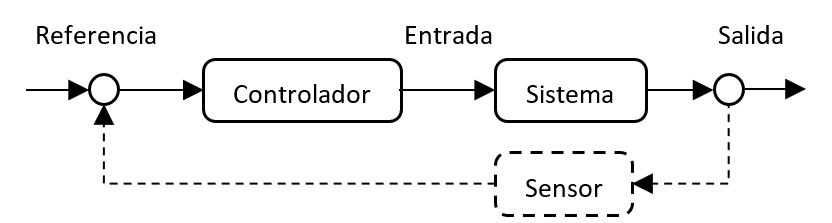
\includegraphics[scale=0.6]{EsquemasControl_ESP.png}
	\caption{Esquema general de control en lazo abierto y control en lazo cerrado. El control en lazo abierto se ilustra con una línea sólida. El control en lazo cerrado se lleva a cabo cuando se incluye el elemento sensor, el cual se ilustra con una línea discontinua. Adaptado de \cite{Wright2016}.}
	\label{Figura: EsqCont}
\end{figure}
\subsection{Control en lazo abierto}
En el control en lazo abierto se genera un comando a la línea de base, esperando que este comando produzca la salida correcta. Aquí no existe una medición de la salida generada, por lo cual tampoco existe alguna medición del error que pudiera utilizarse como mecanismo para la modulación del comando que se genera \cite{Wright2016}.

\subsection{Control en lazo cerrado}
El control en lazo cerrado requiere de la inclusión de algún elemento sensor en el sistema que se desea controlar. Este control retroalimentado genera un comando a la línea de base y el elemento sensor mide la salida del sistema en respuesta al comando. Esta medición de la salida puede utilizarse para determinar diferencias entre la salida esperada y la real, generando así una señal de error que puede utilizarse como retroalimentación hacia el controlador para realizar modificaciones en los comandos generados \cite{Wright2016}.

\subsection{Control adaptativo}
El control adaptativo utiliza sensores para medir la entrada y salida del sistema, utilizando dichas métricas para ajustar el controlador en respuesta a las perturbaciones en el entorno de control o el sistema controlado. Una ventaja de este tipo de control es que se pueden desarrollar estrategias de control sin requerir de un conocimiento completo del sistema que se va a controlar, sin embargo, esto provoca que los controladores adaptativos rara vez sean óptimos \cite{Wright2016}.

\section{Algoritmos de control}
Existe una gran variedad de algoritmos de control que suelen ser usados dentro de las neuroprótesis, sin embargo, para este trabajo sólo se abordaran 3 algoritmos de control.

\subsection{Control On-Off}
El control control On-Off: es una política de control en la que cuando una variable cruza un umbral predefinido, se activa un programa que habilita o deshabilita determinadas funciones del esquema de control \cite{Wright2016}.

\subsection{Máquina de estados finitos (FSM)}
Este es un modelo de sistema que puede considerarse como una implementación más compleja del control on-off. En este modelo, la medición de una variable del sistema en combinación con el estado actual desencadena una serie de acciones y una transición de estado. Este tipo de modelo es periódico, entonces pueden realizarse transiciones de estado en respuesta al tiempo \cite{Wright2016}.

{\color{red}\subsection{Control lineal}}


\section{Retroalimentación}
Como se explicó en la sección 2.3, una señal de retroalimentación es aquella que brinda información al sistema sobre los efectos ante un determinado comando. Estas señales se pueden implementar de más de una forma dentro de una neuroprótesis, por ejemplo, la observación visual de la acción realizado por algún actuador robótico de una una interfaz cerebro-computadora (comúnmente conocido como neurofeedback), la adquisición de una señal bioeléctrica durante un periodo de estimulación eléctrica, o bien la medición de algún elemento sensor que proporcione información sobre el estado del efector o actuador \cite{Wright2016}.

Otro ejemplo de retroalimentación en un sistema de neuroprótesis es el biofeedback, una técnica de retroalimentación donde no se requiere de elemento sensor en el efector o actuador del sistema, ya que consiste en permitir al individuo usuario de la neuroprótesis aprender a cambiar su actividad fisiológica con el fin de mejorar el rendimiento del sistema \cite{Yucha2008}.

\section{Electromiografía de superficie}
La electromiografía se define como la detección y análisis del electromiográma (EMG). El EMG puede detectarse directamente mediante la inserción de electrodos en las fibras musculares, o de forma indirecta colocando electrodos de superficie en las zonas de la piel localizadas justo encima del tejido muscular. A este último método se le suele conocer como electromiografía de superficie (sEMG, por sus siglas en inglés), el cual, al ser un método de detección no invasivo y permitir obtener información sobre la activación muscular, como la intensidad de la contracción muscular, la manifestación de la fatiga muscular y el reclutamiento de unidades motoras, se ha convertido en un método muy popular en la investigación.

\subsection{Procesamiento}
La actividad mioeléctrica en la superficie de la piel se encuentra dentro de un ancho de banda limitado que suele estar desde los 15 hasta los 400 Hz, con amplitudes dentro del rango de micro Volts o mili Volts, dependiendo de la intensidad de la contracción muscular \cite{Cavalcanti-Garcia2009}.

La detección de la actividad mioeléctrica se realiza mediante el uso de un amplificador diferencial, el cual debe tener conectadas las entradas a un par de electrodos situados en la dirección de la fibra muscular a sensar, y además debe tener una referencia situada en el hueso más cercano a la fibra. Una vez detectado de forma eficaz la actividad mioeléctrica, esta debe someterse a un filtro anti-aliasing y posteriorme al proceso de conversión analógico-digital que permitirá se realice el procesamiento digital de la señal \cite{Cavalcanti-Garcia2009}.

Usualmente se suele utilizar un filtro pasa banda con frecuencias de corte similares a las que componen la actividad mioeléctrica (15-400 Hz), acompañado de un filtro notch digital que permita atenuar la interferencia provocada por la línea \cite{Cavalcanti-Garcia2009}.

\subsection{Descriptores de amplitud}
Existen diferentes indicadores que pueden ser utilizados para estimar la amplitud del sEMG, tal es el caso de la amplitud pico a pico, la cual nos proporciona un valor instantaneo de la amplitud del sEMG, sin embargo, no es un indicador de amplitud robusto \cite{Cavalcanti-Garcia2009}.

Los descriptores de amplitud de sEMG más comunes consisten en la promediación de muestras rectificadas o elevadas al cuadrado de sEMG crudo a lo largo de una determinada tarea motora. Estos descriptores son conocidos como el valor rectificado promedio (ARV o MAV, por sus siglas en inglés)(Ecuación \ref{ARV}) y el valor cuadrático medio (RMS, pos sus siglas en inglés)(Ecuación \ref{RMS}). Dichos desciptores suelen ser usados para estimar las variaciones temporales de la amplitud del sEMG en ventanas cortas entre 250 ms o 500 ms \cite{Cavalcanti-Garcia2009}.

\begin{equation}
	ARV = \frac{1}{N} \sum_{n=1}^{N} \abs{EMG[n]}
	\label{ARV}
\end{equation}

\begin{equation}
	RMS = \sqrt{\frac{1}{N} \sum_{n=1}^{N} EMG[n]^{2}}
	\label{RMS}
\end{equation}

Estos descriptores de amplitud suelen proporcionar información similiar, la gran diferencia entre ellos se encuentra en la función de densidad de probabilidad (PDF, por sus siglas en inglés) que generan, donde el RMS suele ser un descriptor con PDF Gaussiana, mientras que el ARV suele ser una descriptor con PDF Laplaciana. En general, se suele utilizar el RMS debido que teóricamente la PDF de sEMG es Gaussiana, sin embargo, existen trabajos que han demostrado que en la práctica la PDF de sEMG es más cercana a una PDF Laplaciana, caso en el cual es recomendable utilizar el ARV como descriptor \cite{Clancy1999}\cite{Phinyomark2013}.